\section{A rational field and two choices of padding}
\label{c:rat-rational}

The equality configuration for the regular tetrahedron uses two
edge-parallel cylinders.  We tilt their axes by a smooth field and
slightly enlarge their parameter domains.  The enlargement must be large
enough to preserve coverage but small enough to be paid for by the decrease
in perpendicular projection area.  The construction below makes this
comparison explicit.

Put $h=1/\sqrt2$ and use the regular edge-one tetrahedron
\begin{equation}\label{c:rat-tetrahedron}
 K_1=\{(x,y,ht):-\tfrac12\le t\le\tfrac12,
       \ |x|\le(\tfrac12+t)/2,\ |y|\le(\tfrac12-t)/2\}.
\end{equation}
Throughout this section write $K=K_1$. Its minimum orthogonal projection area is $h/2$.  We verify this using
Cauchy's projection formula for polytopes, obtained by taking support
functions in the projection-body representation
\cite[equation~(1), p.~83, and Section~3]{Martini1991}.  Its volume is $h/6$, by integration
of the rectangular horizontal sections, and its diameter is one.
For a unit vector $u$, let $d_i$ be the derivatives in direction $u$ of
its four affine barycentric coordinates.  Projecting the entering faces
of the tetrahedron gives
\[
 |\pi_{u^\perp}K|=3\operatorname{vol}(K)\sum_{d_i>0}d_i.
\]
Indeed the inward normal component on the face opposite vertex $v_i$
is $d_i$ times that face's altitude; the projected entering faces
partition the shadow except along projected edges.  Write
$s=\sum_{d_i>0}d_i$.  Since $\sum_i d_i=0$ and
$u=\sum_i d_i v_i$, the vector $u/s$ is a difference of two convex
combinations of the vertices.  The diameter bound gives $s\ge1$.
An edge direction has barycentric derivatives $1,-1,0,0$, proving
$A_{\min}(K)=h/2$.

The equality cover can now be specified explicitly. In the label plane
with coordinates $(Y,T)$, put
\[
 D_0=\{(Y,T):0\le T\le\tfrac12,
                        2|Y|\le\tfrac12-T\}.
\]
The triangle $\{(0,Y,hT):(Y,T)\in D_0\}$, swept parallel to the
$x$-axis, covers the portion $t\ge0$. The reflected triangle
$\{(X,0,-hR):(X,R)\in D_0\}$, swept parallel to the $y$-axis,
covers $t\le0$. Each is already perpendicular to its axis and has
area $h\int_0^{1/2}(1/2-T)\,dT=h/8$, so the total cost is $h/4$.
This is the tetrahedral equality configuration attributed to Bang in
Bezdek's account~\cite[Section~3]{Bezdek2009}.

In the label plane with coordinates $(Y,T)$, write $r=\tfrac12-T$ and set
\[
 \mathcal W=\{(Y,T):r\ge2|Y|\}.
\]
The polynomial $Y^2-r^2/4$ vanishes on both wedge walls.
Dividing it by $r$ produces a potential homogeneous of degree one in $(Y,r)$,
whose gradient depends only on the ratio $Y/r$ away from the apex.
Replacing that denominator by $r+d$ smooths the common apex while
retaining the wall values.  Fix $d>0$ and, on $r>-d$, define
\begin{align}
 \psi(Y,T)&=\frac{Y^2-r^2/4}{4(r+d)}, &
 W_d=(a,b)&=(-\psi_T,\psi_Y),\label{c:rat-potential}\\
 a(Y,T)&=-\frac{Y^2}{4(r+d)^2}
          -\frac{r(r+2d)}{16(r+d)^2}, &
 b(Y,T)&=\frac{Y}{2(r+d)}.\label{c:rat-field}
\end{align}
The standard stream-function form makes the divergence zero and the constant
value of $\psi$ on either wedge wall makes the field tangent to that wall.
We use the straight-line maps $p\mapsto p+\epsilon xW_d(p)$,
not a flow of $W_d$.  The exact derivative identities needed later are
\begin{equation}\label{c:rat-spectrum}
 \operatorname{tr}DW_d=0,\qquad
 \det DW_d=-\frac{d^2}{16(r+d)^4}.
\end{equation}
For example, the $YY,Yr,rr$ derivatives of $\psi$ are
$1/[2(r+d)]$, $-Y/[2(r+d)^2]$, and
$(Y^2/2-d^2/8)/(r+d)^3$.  Their determinant is the one displayed;
replacing $r$ by $\tfrac12-T$ preserves it.

At the dividing level $T=0$, put
\begin{align}
 \alpha&=\frac1{1+2d},&
 c(Y)&=c_0+c_2Y^2=-a(Y,0),\notag\\
 c_0&=\frac{(1/2)(1/2+2d)}{16(1/2+d)^2},&
 c_2&=\frac1{4(1/2+d)^2},&
 P(Y)&=\alpha c(Y)Y^2.\label{c:rat-ceiling-polynomial}
\end{align}
Thus $b(Y,0)=\alpha Y$.  For a positive tilt $\epsilon$ and a
positive padding $q=q(\epsilon)$, use the compact label domain
\begin{equation}\label{c:rat-domain}
 D_{\epsilon,q}=\{(Y,T)\in\mathcal W:T\ge-\tfrac14,
                         \ T\ge-\epsilon^2P(Y)-q\}.
\end{equation}
Figure~\ref{c:fig-equality} shows how this domain extends $D_0$
while retaining the wedge walls.

\begin{figure}[htb]
\centering
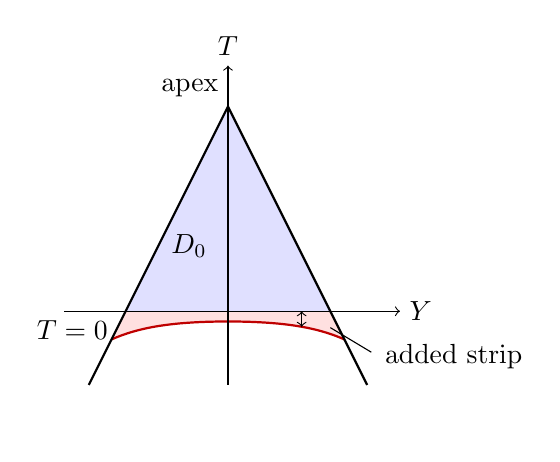
\begin{tikzpicture}[scale=5.2]
 \fill[blue!12] (-.25,0)--(.25,0)--(0,.5)--cycle;
 \begin{scope}
  \clip (-.4,-.3)--(.4,-.3)--(0,.5)--cycle;
  \fill[red!12] (-.34,0)--(.34,0)
    -- plot[domain=.34:-.34,samples=80]
       (\x,{-.025-.3*\x*\x-3*\x*\x*\x*\x}) -- cycle;
  \draw[red!75!black,thick,domain=-.34:.34,samples=80]
    plot (\x,{-.025-.3*\x*\x-3*\x*\x*\x*\x});
 \end{scope}
 \draw[thick] (-.34,-.18)--(0,.5)--(.34,-.18);
 \draw[dashed] (-.25,0)--(.25,0);
 \draw[->] (0,-.18)--(0,.60) node[above] {$T$};
 \draw[->] (-.40,0)--(.42,0) node[right] {$Y$};
 \node[below left] at (-.27,0) {$T=0$};
 \node at (-.095,.16) {$D_0$};
 \node[above left] at (0,.5) {apex};
 \draw[<->] (.18,0)--(.18,-.038);
 \node[right] at (.36,-.11) {added strip};
 \draw[thin] (.35,-.10)--(.25,-.04);
\end{tikzpicture}
\caption{Schematic intercept domain for the first family. The blue
triangle is the unperturbed domain $D_0$; the red strip extends it
below $T=0$. The padded lower boundary ends at the unchanged wedge
walls. Its actual equation is $T=-\epsilon^2P(Y)-q$; the padding is
exaggerated here, and the walls continue below the displayed portion.}
\label{c:fig-equality}
\end{figure}


The two swept sets are
\begin{align}
 S_+&=\{(x,Y+\epsilon xa(Y,T),h(T+\epsilon xb(Y,T))):
                 (Y,T)\in D_{\epsilon,q},\ |x|\le\tfrac12\},\notag\\
 S_-&=\{(X-\epsilon ya(X,R),y,-h(R-\epsilon yb(X,R))):
                 (X,R)\in D_{\epsilon,q},\ |y|\le\tfrac12\}.
 \label{c:rat-sweeps}
\end{align}
For one family, the weighted parameter area is
\begin{equation}\label{c:rat-weighted-cost}
 C_d(\epsilon,q)=h\int_{D_{\epsilon,q}}
          \frac{dY\,dT}{\sqrt{1+\epsilon^2(a^2+h^2b^2)}}.
\end{equation}
This is the quantity in the finite-approximation theorem: the factor $h$
comes from the label plane's physical scale, and the square-root factor
from its orthogonal projection perpendicular to the local line direction.

\begin{proposition}\label{c:rat-rational-proposition}
Fix $d>0$ and a positive function $q(\epsilon)$ such that
$q(\epsilon)=O(\epsilon^2)$ and $\epsilon^3=o(q(\epsilon))$ as
$\epsilon\downarrow0$.  For all sufficiently small $\epsilon>0$,
\[
 K\subset S_+\cup S_-.
\]
Moreover, with
\[
 D_0=\mathcal W\cap\{T\ge0\},\quad
 J_d=\int_{-1/4}^{1/4}P(Y)\,dY,\quad
 I_d=\frac12\int_{D_0}(a^2+h^2b^2)\,dY\,dT,
\]
one has
\begin{equation}\label{c:rat-cost-expansion}
 \frac{C_d(\epsilon,q)}h
   =\frac18+\epsilon^2(J_d-I_d)+\frac q2+O(\epsilon^4).
\end{equation}
The remainder constant may depend on $d$ and on a fixed bound for
$q/\epsilon^2$.  The coverage threshold may also depend on the rate
at which $\epsilon^3/q$ tends to zero.  Finally,
\begin{equation}\label{c:rat-coefficient-limits}
 \lim_{d\downarrow0}J_d=\frac{16}{15360},\qquad
 \lim_{d\downarrow0}I_d=\frac{17}{15360}.
\end{equation}
\end{proposition}

We first establish coverage, including the wedge walls.  We then compare
the area added to the label domain with the area saved by tilting the
axes.  Keeping $d$ fixed throughout these two arguments is essential:
the limiting field at $d=0$ is used only to evaluate coefficient limits.

\subsection{Inverting the tilted maps}
\label{c:rat-inverse}

We first obtain inverse labels anywhere in the wedge; the next
subsection tests their lower-boundary inequalities. For fixed $d$, both
$W_d$ and $DW_d$ are bounded on the entire wedge.
For $|x|\le\tfrac12$, consider
\[
 F_x(Y,T)=(Y,T)+\epsilon xW_d(Y,T).
\]
We claim that $F_x$ maps $\mathcal W$ onto itself for all sufficiently
small $\epsilon$, uniformly in $x$.  The same statement holds with
$-\epsilon$.

The wall functions $r/2\pm Y$ change by
$\epsilon x(-b/2\pm a)$.  Each latter expression vanishes on the
corresponding wall and has bounded $Y$-derivative.  Moving horizontally
from that wall gives
\[
 |-b/2\pm a|\le C_d(r/2\pm Y)\quad\text{on }\mathcal W.
\]
For small $\epsilon$, therefore, each wall function retains its sign
and vanishes precisely on the same wall.  The interior maps into the
interior and the boundary into the boundary.  Also
\[
 \det DF_x=1+\epsilon^2x^2\det DW_d>0
\]
uniformly on the wedge, so the image of its interior is open by the
inverse function theorem.  The image of the closed wedge is closed:
a convergent sequence of images has bounded preimages because the
displacement is bounded, and hence has a convergent subsequence of
preimages in the wedge.  Boundary points cannot map to the interior.
Consequently the interior image is also closed relative to the
connected wedge interior.  It is nonempty, so it is the whole interior;
closedness supplies the boundary.  This proves the claim.

\subsection{Why the two families leave no gap}
\label{c:rat-overlap}

For $(x,y,ht)\in K$, both $(y,t)$ and $(x,-t)$ lie in $\mathcal W$.
The preceding surjectivity supplies wedge labels satisfying
\begin{align*}
 y&=Y+\epsilon xa(Y,T),&t&=T+\epsilon xb(Y,T),\\
 x&=X-\epsilon ya(X,R),&-t&=R-\epsilon yb(X,R).
\end{align*}
If either label belongs to $D_{\epsilon,q}$, the point is covered.
Suppose both labels fail.  Since $P$ and $q$ are nonnegative, this
forces $T,R<0$.  Boundedness of $W_d$ first gives
$|t|,|T|,|R|=O(\epsilon)$ and $Y=y+O(\epsilon)$,
$X=x+O(\epsilon)$.  All remainders below are uniform over $K$.
Since $b(Y,0)=\alpha Y$,
\[
 T=t-\epsilon\alpha xy+O(\epsilon^2),\qquad
 R=-t+\epsilon\alpha xy+O(\epsilon^2).
\]
Their sum is $O(\epsilon^2)$ and both are negative, so separately
$T,R=O(\epsilon^2)$.  The smooth formulas now give
\begin{align*}
 Y&=y+\epsilon xc(y)+O(\epsilon^2),&
 X&=x-\epsilon yc(x)+O(\epsilon^2),\\
 b(Y,T)&=\alpha y+\epsilon\alpha xc(y)+O(\epsilon^2),&
 b(X,R)&=\alpha x-\epsilon\alpha yc(x)+O(\epsilon^2).
\end{align*}
Thus
\begin{equation}\label{c:rat-inverse-sum}
 T+R=-\epsilon^2\alpha\bigl(x^2c(y)+y^2c(x)\bigr)+O(\epsilon^3).
\end{equation}
The choice of $P$ is explained by the exact identity
\begin{equation}\label{c:rat-square-surplus}
 P(x)+P(y)-\alpha\bigl(x^2c(y)+y^2c(x)\bigr)
       =\alpha c_2(x^2-y^2)^2\ge0.
\end{equation}
Replacing $x,y$ by $X,Y$ in $P$ changes it by $O(\epsilon)$.
Equation~\eqref{c:rat-inverse-sum} therefore gives
\[
 T+R\ge-\epsilon^2(P(X)+P(Y))-C\epsilon^3.
\]
The cutoff at $-1/4$ cannot fail when $T,R=O(\epsilon^2)$.
Failure of both remaining domain inequalities would give instead
\[
 T+R<-\epsilon^2(P(X)+P(Y))-2q.
\]
This contradicts $\epsilon^3=o(q)$.  The two families therefore cover
all of $K$, including the boundary points handled by the inverse maps.

\subsection{The area comparison and finite choices}
\label{c:rat-area}

We now prove the cost assertions in Proposition~\ref{c:rat-rational-proposition}.
The unperturbed label domain $D_0$ has area $1/8$.  For
$|Y|\le1/4$, the added interval below $T=0$ has length exactly
$\epsilon^2P(Y)+q$ for small $\epsilon$.  Outside that interval of
$Y$-values, both the width and depth of the added portion are
$O(\epsilon^2)$, because $q=O(\epsilon^2)$ and $P$ is bounded on
$|Y|\le3/8$.  Hence
\[
 |D_{\epsilon,q}|=\frac18+\epsilon^2J_d+\frac q2+O(\epsilon^4).
\]
The field is bounded on these domains.  Taylor expansion of the
integrand in \eqref{c:rat-weighted-cost} has uniform remainder
$O(\epsilon^4)$, and replacing the domain of its quadratic term by
$D_0$ changes that term by $O(\epsilon^4)$.  This proves
\eqref{c:rat-cost-expansion} with its stated remainder.

For the coefficient comparison we may now let $d\downarrow0$.
On $T=0$ one has
$P(Y)\to(1/16+Y^2)Y^2$, giving
\[
 J_d\longrightarrow\int_{-1/4}^{1/4}(Y^2/16+Y^4)\,dY
                 =\frac1{960}.
\]
On $D_0$, write $z=Y/r$ away from the apex.  Then $|z|\le1/2$,
$a\to-(1/16+z^2/4)$ and $b\to z/2$.  The fields are uniformly
bounded there for $d>0$, so bounded convergence and $dY\,dT=r\,dz\,dr$
yield
\[
 I_d\longrightarrow\frac12\int_0^{1/2}r\,dr
     \int_{-1/2}^{1/2}
      \left[\left(\frac1{16}+\frac{z^2}4\right)^2
                     +\frac12\left(\frac z2\right)^2\right]dz
     =\frac{17}{15360}.
\]
This completes the proof of Proposition~\ref{c:rat-rational-proposition}.

There are two useful parameter schedules.  First choose $d>0$ with
$\Delta_d=I_d-J_d>0$.
For \emph{vanishing padding}, take $q=\epsilon^{5/2}$; then
\[
 C_d(\epsilon,\epsilon^{5/2})/h
       =\frac18-\Delta_d\epsilon^2+o(\epsilon^2)<\frac18
\]
for all sufficiently small positive $\epsilon$.
For \emph{fixed quadratic padding}, choose $\eta>0$ with
$\eta/2<\Delta_d$, keep it fixed, and take $q=\eta\epsilon^2$.
In this case the sharper expression is
\[
 C_d(\epsilon,\eta\epsilon^2)/h
       =\frac18-(\Delta_d-\eta/2)\epsilon^2+O(\epsilon^4)<\frac18.
\]
The parameter order is respectively $d,\epsilon$ or $d,\eta,\epsilon$.

For either schedule, fix such a positive $\epsilon$.
The label domain is compact, and the field is smooth on a neighborhood
of it.  The eigenvalues of $D(\pm\epsilon W_d)$ are
\[
 \pm\frac{\epsilon d}{4(r+d)^2}.
\]
Since $d$ was fixed first, their magnitudes times the axial half-length
$1/2$ are strictly below one when $\epsilon$ is small.
Apply \BScaling{} with $V=+\epsilon W_d$
for $S_+$, and with $V=-\epsilon W_d$ followed by the isometry
$(x,y,z)\mapsto(y,x,-z)$ for $S_-$.  Each application gives finitely
many cylinders with cost at most $C_d(\epsilon,q)+e$.  Choose the sum of the two errors less than
$h/4-2C_d(\epsilon,q)>0$.  Together the finite covers cover $K$ and
have total cost less than $h/4=A_{\min}(K)/2$.
The approximation theorem gives compact parallelogram bases.  Enlarging
them slightly in their own perpendicular planes also gives bounded
open parallelogram bases, with the total added area chosen smaller
than the remaining strict slack.  No mesh uniform in $\epsilon$ is
needed.  Similarity scales every base area and the minimum projection
area by the same factor, proving Theorem~\ref{c:main}
for every positive edge length.
